\section{When does fusion improve on RGB?}
\label{sec:late-transfer}
\cohortline{CORRECTED TRANSFER / \AuditTransferCount{} eligible of 508 candidates / 32 development-exposed sequences / supplied ROI}

The frozen-modality comparison tests whether the shared phase interface improves errors in seconds beyond the benchmark setting. Fusion has lower point MAE and p95 than RGB alone on the revised cohort, whereas RGB retains lower median and relative error. Paired sequence-bootstrap intervals for mean, median, and p95 differences include zero.

\subsection{Evaluation population}
We evaluate frozen predictions on \AuditTransferCount{} eligible queries from 32 EvTTC sequences. The registered sampling contains 508 candidate queries; eligibility requires a public TTC label within 50\,ms of the query, with ties assigned to the earlier timestamp. All eligible targets are positive. The primary annotated object supplies the query region. These sequences had been used during development, as specified in Section~\ref{sec:protocol}.

A source audit identified a reversed low/medium target assignment for two recordings in our earlier analysis. Matching the public download identities and source hashes corrected this association without changing sensor queries or predictions. We report only the corrected cohort here; Appendix~\ref{app:target-association} records all candidate counts, exclusions, and the superseded assignment.

\subsection{Corrected error distribution}
Relative time error remains $100|\widehat T-T|/|T|$. Pooled summaries weight queries equally; sequence-macro summaries weight each sequence group equally. Temporal support differs across complete systems: PHASE-TTC uses up to 650\,ms of history, while Garl uses two observations separated by 0.1\,s.

\begin{table}[htbp]
\centering\small
\resizebox{\linewidth}{!}{%
\begin{tabular}{lrrrrrrr}
\toprule
Cohort / model & $n$ & MAE & Median & p95 & RTE (\%) & Macro MAE & Macro RTE (\%) \\
\midrule
Corrected extended: PHASE-TTC & 460 & 0.813 & 0.446 & 2.742 & 29.112 & 0.827 & 30.016 \\
Corrected extended: RGB context & 460 & 0.851 & 0.390 & 3.038 & 29.017 & 0.859 & 29.368 \\
Corrected extended: Event context & 460 & 1.376 & 0.844 & 3.707 & 58.154 & 1.377 & 57.764 \\
Corrected extended: Garl full & 460 & 3.166 & 0.635 & 4.781 & 131.268 & 3.041 & 126.366 \\
Historical46: PHASE-TTC & 46 & 0.141 & 0.136 & 0.250 & 7.748 & 0.159 & 8.419 \\
Historical46: RGB context & 46 & 0.113 & 0.099 & 0.264 & 6.387 & 0.114 & 6.246 \\
Historical46: Event context & 46 & 0.286 & 0.241 & 0.692 & 15.822 & 0.289 & 15.566 \\
Historical46: Garl full & 46 & 0.250 & 0.186 & 0.561 & 13.327 & 0.282 & 14.649 \\
\bottomrule
\end{tabular}
}
\caption{Corrected-label transfer: 460 eligible of 508 extended candidates across 32 sequences. Historical46 remains separate (46 queries, three sequences). Absolute errors are seconds; macro gives equal weight to sequences.}
\label{tab:audit-transfer-summary}
\end{table}


Fusion MAE is \AuditFusionMAE{}\,s against RGB's \AuditRgbMAE{}\,s; its empirical p95 is \AuditFusionPninetyfive{}\,s against \AuditRgbPninetyfive{}\,s. RGB retains lower median error, \AuditRgbMedian{} versus \AuditFusionMedian{}\,s, and slightly lower RTE, \AuditRgbRTE{} versus \AuditFusionRTE{}.  \evidence{GT01}

\begin{figure}[H]
\centering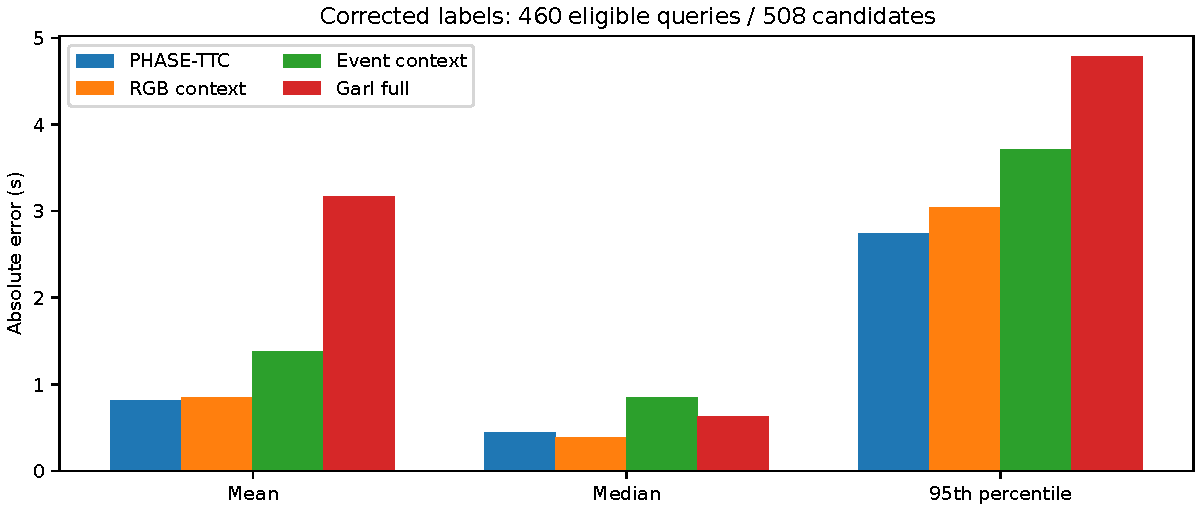
\includegraphics[width=.94\linewidth]{figures/audit_transfer_summary.pdf}
\caption{\textbf{Corrected frozen-transfer error summaries.} PHASE-TTC and RGB use the same \AuditTransferCount{} eligible queries after reassociating all 508 candidates. Lower point mean and p95 favor fusion; lower median favors RGB. Paired intervals are reported separately in Table~\ref{tab:audit-transfer-bootstrap}.}
\label{fig:transfer-tradeoff}
\end{figure}

\subsection{Exceedance and paired uncertainty}
The full corrected distribution retains signed predictions, including large errors. Figure~\ref{fig:transfer-exceedance} shows the fraction at or above each absolute-error threshold. Maximum absolute error is \AuditFusionMax{}\,s for fusion and \AuditRgbMax{}\,s for RGB. These are query-level errors under the corrected labels, not scorer-defined invalid predictions.

\begin{figure}[htbp]
\centering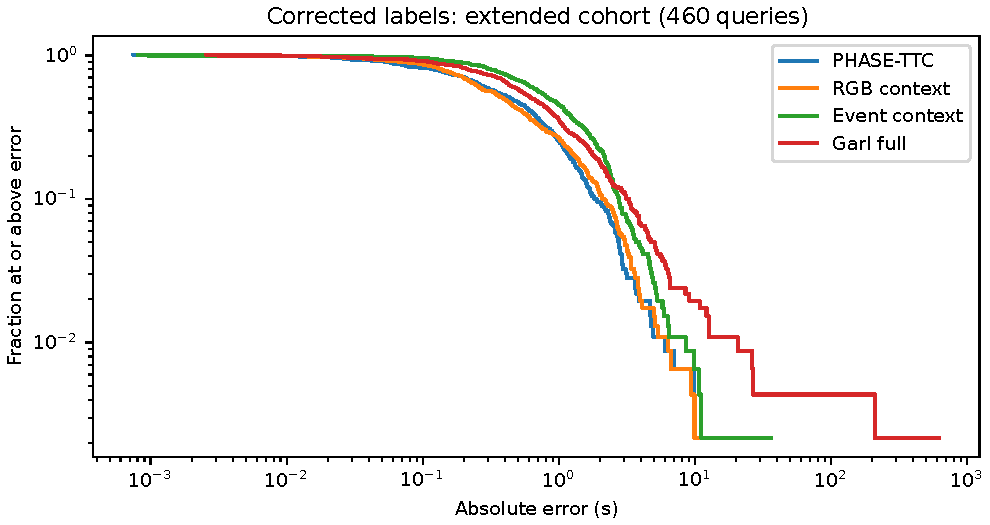
\includegraphics[width=\linewidth]{figures/audit_transfer_exceedance.pdf}
\caption{\textbf{Corrected absolute-error exceedance.} Curves include all \AuditTransferCount{} eligible transfer queries with equal query weights. No signed prediction is clipped and no extreme error is removed.}
\label{fig:transfer-exceedance}
\end{figure}

The PHASE-minus-RGB mean difference is \AuditMeanDelta{}\,s with interval $[\AuditMeanLow,\AuditMeanHigh]$\,s; the p95 difference is \AuditPninetyfiveDelta{}\,s with interval $[\AuditPninetyfiveLow,\AuditPninetyfiveHigh]$\,s. All three paired intervals include zero. The procedure uses 10,000 complete-sequence resamples with linear quantiles and the same frozen models. Appendix~\ref{app:derived-transfer} gives complete sequence results and distinguishes this corrected analysis from the historical one.
\begin{table}[htbp]
\centering\small
\resizebox{\linewidth}{!}{%
\begin{tabular}{lllrr}
\toprule
Cohort & Paired contrast & Estimand & Difference & 95\% interval \\
\midrule
Extended460 & PHASE minus RGB & mean & -0.038 & [-0.147, +0.061] \\
Extended460 & PHASE minus RGB & median & +0.055 & [-0.042, +0.136] \\
Extended460 & PHASE minus RGB & p95 & -0.296 & [-0.657, +0.193] \\
Extended460 & PHASE minus Garl & Macro MAE\_s & -2.214 & [-4.951, -0.447] \\
Extended460 & PHASE minus Garl & Macro RTE\_pct & -96.350 & [-211.946, -16.629] \\
Historical46 & PHASE minus RGB & mean & +0.028 & [+0.005, +0.103] \\
Historical46 & PHASE minus RGB & median & +0.036 & [+0.026, +0.068] \\
Historical46 & PHASE minus RGB & p95 & -0.014 & [-0.098, +0.109] \\
Historical46 & PHASE minus Garl & Macro MAE\_s & -0.123 & [-0.178, -0.084] \\
Historical46 & PHASE minus Garl & Macro RTE\_pct & -6.230 & [-8.682, -4.767] \\
\bottomrule
\end{tabular}
}
\caption{Whole-sequence paired percentile intervals. PHASE--RGB uses 10,000 draws, seed 20261028, for pooled query errors; PHASE--Garl uses 2,000 draws, seed 7, for equal-sequence means. Linear quantiles; negative favors PHASE. MAE, median and p95 use seconds; RTE uses percentage points. Exposed development cohorts.}
\label{tab:audit-transfer-bootstrap}
\end{table}

\FloatBarrier
